% Chapter Template

\chapter{Experimento: Buscando el Efecto Espejo en una tarea Perceptual} % Main chapter title

\label{Cap_Exp} % Change X to a consecutive number; for referencing this chapter elsewhere, use \ref{ChapterX}

%----------------------------------------------------------------------------------------
%	SECTION 1
%----------------------------------------------------------------------------------------
\section{Planteamiento general}

%Se propone buscar evidencia del Efecto Espejo en una tarea fuera de Memoria de reconocimiento


%Se propone una tarea perceptual ya que carece de una fase de preparacion
El interés principal del trabajo aquí expuesto es evaluar la posibilidad de que el Efecto Espejo y los patrones de respuesta reportados en estudios de memoria de reconocimiento como parte del mismo, sean producto de la aplicación del modelo de detección de señales en la comparación del desempeño de los participantes en dos condiciones de dificultad (i.e. dos niveles de d') y no así de una discrepancia a nivel de procesos superiores de atención, procesamiento y memoria que determine la distribución de dichos grupos de estímulos en el eje de la evidencia. Para ello se diseñó una tarea de detección meramente perceptual, donde las condiciones de dificultad fueron construidas con base en su discriminabilidad perceptual.\\ 

%Se trabaja con ilusiones opticas, dado que la literatura en ellas permite anticiparnos a la d' y proponer dos niveles de dificultad.
Las ilusiones ópticas 

\subsection{Objetivo}

%Buscar evidencia del efecto espejo en una tarea de detección que no implique el reconocimiento de estimulos ya conocidos.
Poner a prueba la existencia de los patrones de respuesta identificados como parte del Efecto Espejo en una tarea de detección perceptual con dos niveles de dificultad, (i.e. una tarea de detección que no pertenezca a la familia de tareas de reconocimiento y, principalmente, que carezca de una etapa previa a la fase experimental donde los participantes tuvieran ocasión de manipular los estímulos y dar un trato distinto a cada nivel de dificultad).\\

\section{Construcción de los Experimentos}

%La tarea de detección princiál consiste en comparar el tamaño de dos círculos en pantalla, donde uno de ellos o ambos podía estar construido como una Figura de Ebbinghaus (dependiendo del Experimento)
Para poner a prueba la extensión del Efecto Espejo a fenómenos más allá de la memoria de reconocimiento, se diseñó una tarea de detección perceptual donde el objetivo de los participantes era señalar aquellos ensayos en que dos círculos a comparar fueran del mismo tamaño, indicando si éste era el caso ensayo a ensayo presionando una de dos posibles teclas. Se construyeron dos variaciones de esta tarea donde, para controlar la dificultad de la tarea, solo uno de estos circulos, o ambos, fueron construidos como parte de una figura de Ebbinghaus (variaciones a las cuales nos referiremos como Experimento 1 y Experimento 2, respectivamente).\\ 

%Descripcion de la Ilusión de Ebbinghaus, la composición de la figura y cómo se explica.
La ilusión de Ebbinghaus (a.k.a. Círculos de Titchner) refiere a un fallo en la estimación del tamaño de un círculo cuando este aparece rodeado por un halo de círculos uniformes de mayor o menor tamaño (Ver Figura~\ref{fig:Ebbinghaus}). La ilusión suele explicarse como producto de la interferencia producida por la estructura de los estímulos sobre el sistema cognoscitivo-perceptual que estima el tamaño de los estímulos en relación a cómo contrastan éstos con su entorno ($REFERENCIA$). De tal forma que la ilusión de Ebbinghaus comprende dos posibles efectos sobre la estimación del tamaño del círculo central: la subestimación y la sobrestimación; la primera de ellas, refiere a cuando el círculo central se encuentra rodeado por un halo de círculos de mayor tamaño que inducen la subestimación de su tamaño y, la segunda, implica el caso contrario en que los círculos externos son más pequeños que el círculo central y llevan al espectador a percibir a este último como más grande de lo que en realidad es.\\

\begin{figure}[th]
\centering

\includegraphics[width=0.55\textwidth]{Figures/Ebbinghaus} 
\decoRule
\caption[Ilusión de Ebbinghaus ejemplar]{Ilustración de la Ilusión de Ebbinghaus. Los círculos centrales de ambas figuras son del mismo tamaño. Sin embargo, el círculo central de la figura izquierda tiende a ser percibido como más pequeño (efecto de subestimación) y el círculo derecho suele ser percibido como más grande (efecto de sobrestimación), como producto del contraste que guardan con los círculos circundantes.}
\label{fig:Ebbinghaus}
\end{figure}

%Factores o variables que han demostrado influir en la intensidad de la ilusión.
La intensidad de la ilusión de Ebbinghaus (i.e. la desviación inducida en la estimación del tamaño del círculo central en relación a su tamaño real) está relacionada con tres variables: 

\begin{itemize}
\item El tamaño de los círculos externos.
\item La distancia entre el círculo central y el halo de círculos externos.
\item El número de círculos externos.
\end{itemize}

%Descripción del procedimiento empleado por Massaro y Anderson para probar la influencia del numero de circulos externos y el tamaño de los mismos en la Ilusión de Ebbinghaus.
La Figura~\ref{fig:Ebb_Var} muestra los resultados de uno de los experimentos conducidos por \parencite{Massaro1971} para evaluar el efecto de las variables involucradas en las figuras de Ebbinghaus en la magnitud de la ilusión. Para dicho experimento, se trabajó con figuras de Ebbinghaus construidas con un diseño factorial de 2x3x5: dos posibles tamaños del círculo central (13 y 17 mm); tres niveles de 'número de círculos externos' (dos, cuatro y seis); cinco niveles del tamaño de los círculos externos que diferían del círculo central en -8, -4, 0, 4 y 8 mm; la distancia entre el círculo central y los externos se mantuvo constante para todas las figuras. Por cada figura de Ebbinghaus presentada, los participantes tenían que elegir de entre un set de círculos de comparación aquel cuyo diámetro se aproximara más al círculo central de la figura de Ebbinghaus (i.e. 27 círculos aislados que variaban en tamaño dentro de un rango  de 8.5 a 21.5 mm en saltos de 0.5 mm).\\

%Descripción de los resultados encontrados por Massaro y Anderson en el mismo estudio.
La figura~\ref{fig:Ebb_Var} reportada por \parencite{Massaro1971} muestra el diámetro promedio del círculo de comparración elegido como 'igual' al círculo central de las figuras de Ebbinghaus (los autores promediaron entre ambos valores de círculo central), a lo largo de los distintos niveles de número de círculos externo, por cada tamaño implementado de círculos externos. El efecto de ambas variables se muestra de manera clara: mientras más círculos externos se presentan en la figura de Ebbinghaus, mayor es la intensidad de la ilusión (i.e. aumenta la distancia entre el valor real del tamaño del círculo central y la estimación de los participantes), como se puede observar en la tendencia que siguen las pendientes; mientras mayor sea la diferencia entre el tamaño del círculo central y los círculos externos, la ilusión aparece con mayor intensidad, como se puede observar por la distancia vertical que separa cada una de las líneas trazadas. En la figura se puede distinguir claramente entre el efecto de sobreestimación (inducido por las figuras cuyos círculos externos eran más pequeños que el círculo central), y subestimación, (donde las figuras tienen círculos externos más grandes que el círculo central). \\

\begin{figure}[th]
\centering
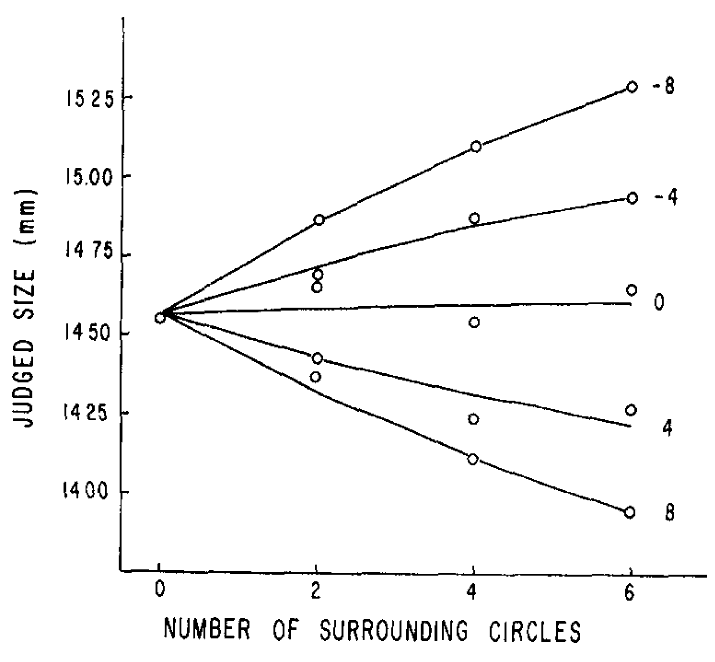
\includegraphics[width=0.55\textwidth]{Figures/Ebb_Variables} 
\decoRule
\caption[Efecto del Numero y Tamaño de los círculos externos en la Ilusión de Ebbinghaus]{Se muestra el efecto que tienen el número de círculos externos incluídos en la ilusión de Ebbinghaus (eje x) sobre los fallos en la estimación del tamaño del círculo central (eje Y); se muestran con líneas diferentes los resultados obtenidos por ilusiones de Ebbinghaus donde los círculos externos diferían en tamaño del círculo central con los valores especificados. La figura fue extraída de la investigación conducida por \parencite{Massaro1971}; Figura 2}
\label{fig:Ebb_Var}
\end{figure}

%Las condiciones de dificultad estarán determinadas por el número de círculos externos
De acuerdo con los hallazgos reportados por \parencite{Massaro1971}, se decidió trabajar con el número de círculos externos como factor determinante para la construcción de dos niveles de d'. La tarea de detección propuesta contaría con una condición fácil (i.e. D' mayor) donde las figuras de Ebbinghaus estuvieran compuestas por pocos círculos externos (2 o 3 círculos) y una condición difícil (i.e. D' menor) con más círculos externos (7 u 8 círculos externos).\\ 

\subsection{Diseño de los Estímulos}

%En el experimento se trabajó con figuras de Ebbinghaus que promovieran efecto de subestimación Y sobrestimación del tamaño. 
Las figuras de Ebbinghaus diseñadas para los experimentos propuestos incluían los dos tipos de ilusiones. Se construyeron figuras que favorecían la sobrestimación y la subestimación utilizando dos tamaños fijos para los círculos externos (5 cm y 1 cm, respectivamente). El tamaño de los círculos externos en las figuras de subestimación (5 cm) se eligió de manera tal que estos fueran más grandes que todos los tamaños de círculo central empleados (entre 1 y 3 cm, en saltos de 0.5 cm). El tamaño utilizado para las figuras de sobreestimación (1cm) se eligió procurando que los circulos externos fueran más pequeños que la mayoría de los círculos centrales a utilizar. Arbitrariamente, dada la configuración de la pantalla a utilizar para correr los experimentos, se decidió sacrificar la relación con el círculo central más pequeño (también de 1cm de diámetro), cancelando -en teoría- la existencia de cualquier efecto sobre la estimación de su tamaño. La razón por la que se incluyeron tanto figuras con efecto de sobrestimación como subestimación fue la de prevenir la habituación y la fatiga de los participantes durante la tarea, dotándole de cierto dinamismo con una mayor variabilidad en los estímulos presentados. Los tamaños de círculos externos propuestos se mantuvieron constantes a lo largo de los distintos niveles de 'número de círculos externos' en cada condición. Dado que el objetivo principal de la esta investigación es comparar el desempeño de los participantes entre las condiciones de dificultad propuestas, el posible efecto diferencial que pudieran tener los tamaños de círculos externos elegidos en su interacción con los tamaños de círculo central probados no se controló en el diseño de las figuras dado que esta relación permaneció constante entre las condiciones a comparar.\\

%No se controló la distancia entre el círculo central y los círculos externos.
En ninguno de los experimentos realizados se controló la distancia entre el círculo central y el halo de círculos externos. Al construir las figuras de Ebbinghaus el halo de círculos externos se formó de acuerdo al número de círculos externos, comenzando con las figuras de la condición difícil que contenían entre 7 y 8 círculos externos. Una vez habiendo distribuido los 7 u 8 círculos externos de manera equidistante entre sí en torno al círculo central, se usaron estas mismas figuras como base para la construcción de estímulos de la condición fácil con 2 o 3 círculos externos, borrando los círculos sobrantes y respetando la ubicación de los restantes respecto del círculo central; para las figuras con 2 círculos externos, se procuró que estos estuvieran enfrentados en puntos opuestos del círculo central y para las figuras con tres círculos centrales se procuró que estos estuvieran localizados de manera tal que formasen un ángulo de $120°$ entre sí. El tamaño impuso una restricción importante en la formación de estos halos de 7 u 8 círculos externos, por lo que su localización permaneció constante a lo largo de los distintos tamaños de círculo central, modificando en consecuencia la distancia entre estos. Es en este sentido que se habla de una falta de control en la distancia entre los círculos centrales y el halo de círculos externos. Sin embargo, apelando nuevamente a que dichas distancias permanecen constantes entre condiciones de dificultad, no se consideró una fuente de ruido importante para analizar lo que se propuso en la tarea: diferencias en el desempeño dependientes del número de círculos externos.\\

A continuación, se desarrolla con detalle la construcción de los estímulos (Señales y ruido) utilizados en cada uno de los dos experimentos realizados.\\

\begin{itemize}
\item Experimento 1 : Circulo de referencia aislado vs Figura de Ebbinghaus.

%Los ensayos de la tarea de detección están compuestos por un círculo aislado constante del lado izquierdo, cuyo tamaño debe ser comparado con el círculo central de una figura de Ebbinghaus en el lado derecho de la pantalla.
En el Experimento 1 sólo se mostraba una figura de Ebbinghaus por ensayo, siempre en la mitad derecha de la pantalla, cuyo círculo central los participantes tenían que comparar con un círculo de referencia de 2 cm de diámetro, con localización fija en la mitad izquierda de la pantalla, para determinar si su tamaño era el mismo (señal) o no (ruido). Los círculos a comparar aparecían a la misma altura de la pantalla y a la misma distancia del centro de la pantalla.\\

%Desarrollo del diseño factorial de 5x2x2 utilizado para construir los estímulos del Experimento 1.
Las figuras de Ebbinghaus utilizadas en el Experimento 1 se diseñaron de acuerdo a un diseño factorial de 5x2x2, (Ver Figura~\ref{fig:Exp_1}). Se utilizaron cinco diferentes tamaños de círculo central, partiendo del tamaño del círculo de referencia (2 cm; la combinación con la señal) y alejándose de este en saltos de 0.5 cm en ambas direcciones (i.e. Círculos más pequeños que la referencia, de 1 y 1.5 cm, y círculos más grandes que la referencia, de 2.5 y 3 cm de diámetro). Por cada uno de estos cinco tamaños de círculo central, se construyeron dos tipos de figuras de Ebbinghaus dependientes del tamaño de los círculos externos: grande (efecto de subestimación) y pequeño (efecto de sobrestimación). Por último, por cada una de estas 10 combinaciones, se hicieron dos figuras diferentes de acuerdo a los niveles de 'número de círculos externos' propuestos por condición (2 y 3 círculos en la condición fácil; 7 y 8 círculos en la condición difícil). Esto nos deja con un subtotal de 20 figuras diferentes por condición y un total de 40 en todo el experimento.\\
 
%Los estímulos con ruido se presentaron 10 veces durante el experimento. Los estímulos con señal se presentaron con 40 repeticiones. La discrepancia en el número de repeticiones entre ambos tipos de estímulo se hizo para igualar la  
El set de figuras de Ebbinghaus construido contiene una mayor cantidad de estímulos con ruido (32 figuras con ruido; 16 por condición) que con la señal (8 figuras con la señal; 4 por condición). 

\begin{figure}[th]
\centering
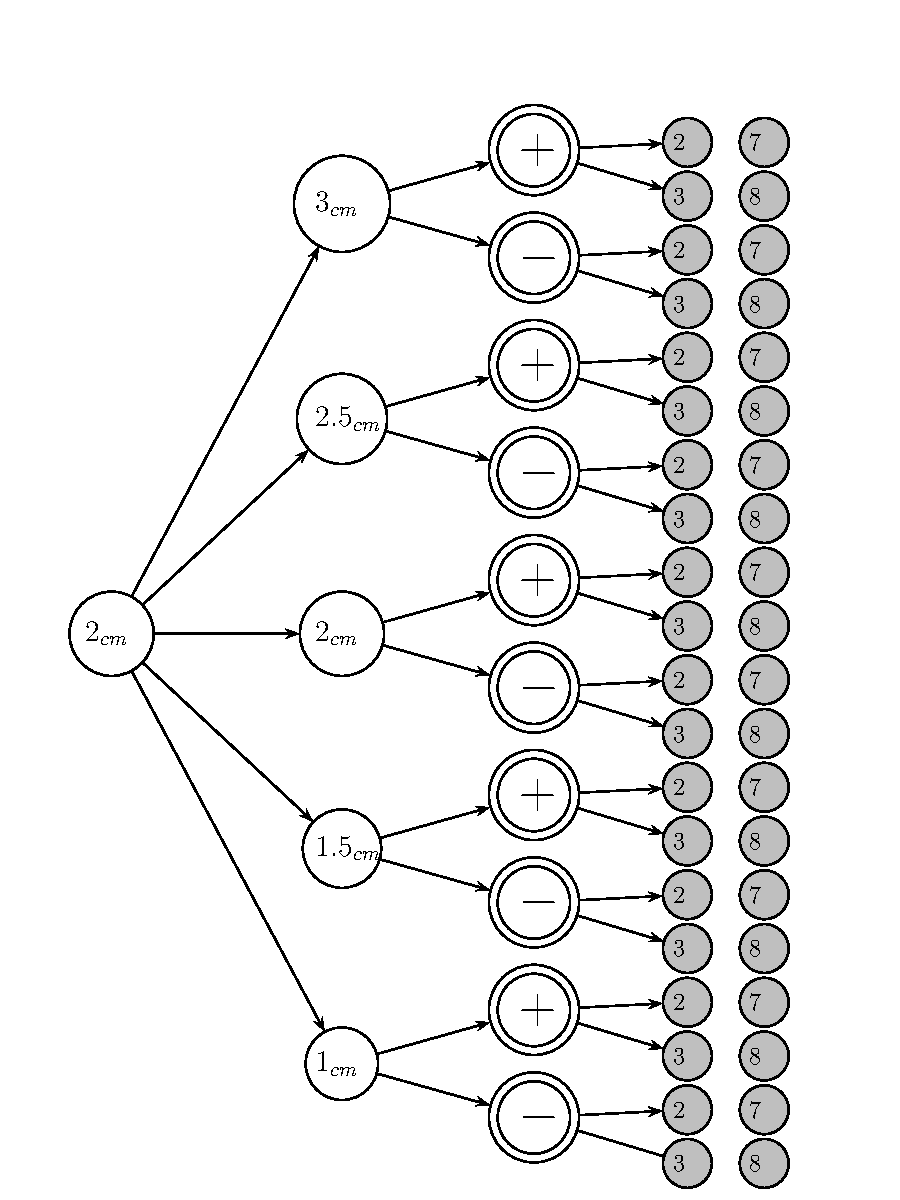
\includegraphics[width=0.99\textwidth]{Figures/Estimulos_Experimento1} 
\decoRule
\caption[Diseño de Estimulos en el Experimento 1]{Diseño factorial (5x2x2) utilizado para construir los estímulos utilizados durante la tarea de detección en el Experimento 1. En cada ensayo los participantes tenían que comparar el tamaño de un círculo de referencia constante con el círculo central de una figura de Ebbinghaus, que podía aparecer en cinco posibles tamaños, con círculos externos que inducen efectos de sobrestimación o subestimación (indicado en el esquema con  y signos positivos y negativos, respectivamente) y con dos niveles de 'número de círculos externo' por condición (2 y 3 círculos externos en la condición fácil o 7 y 8 en la condición difícil). Por cada condición de dificultad, se tienen 16 estímulos con ruido, (10 repeticiones por cada uno, en cinco colores diferentes) y 4 que contienen la señal (repetidos 40 veces cada una, en cinco colores diferentes), dejándonos con 320 ensayos por condición y un total de 640 ensayos en el experimento.}
\label{fig:Exp_1}
\end{figure}



\item Experimento 2 : Figura de Ebbinghaus (Sobrestimación) vs Figura de Ebbinghaus (Subestimación).



\begin{figure}[th]
\centering
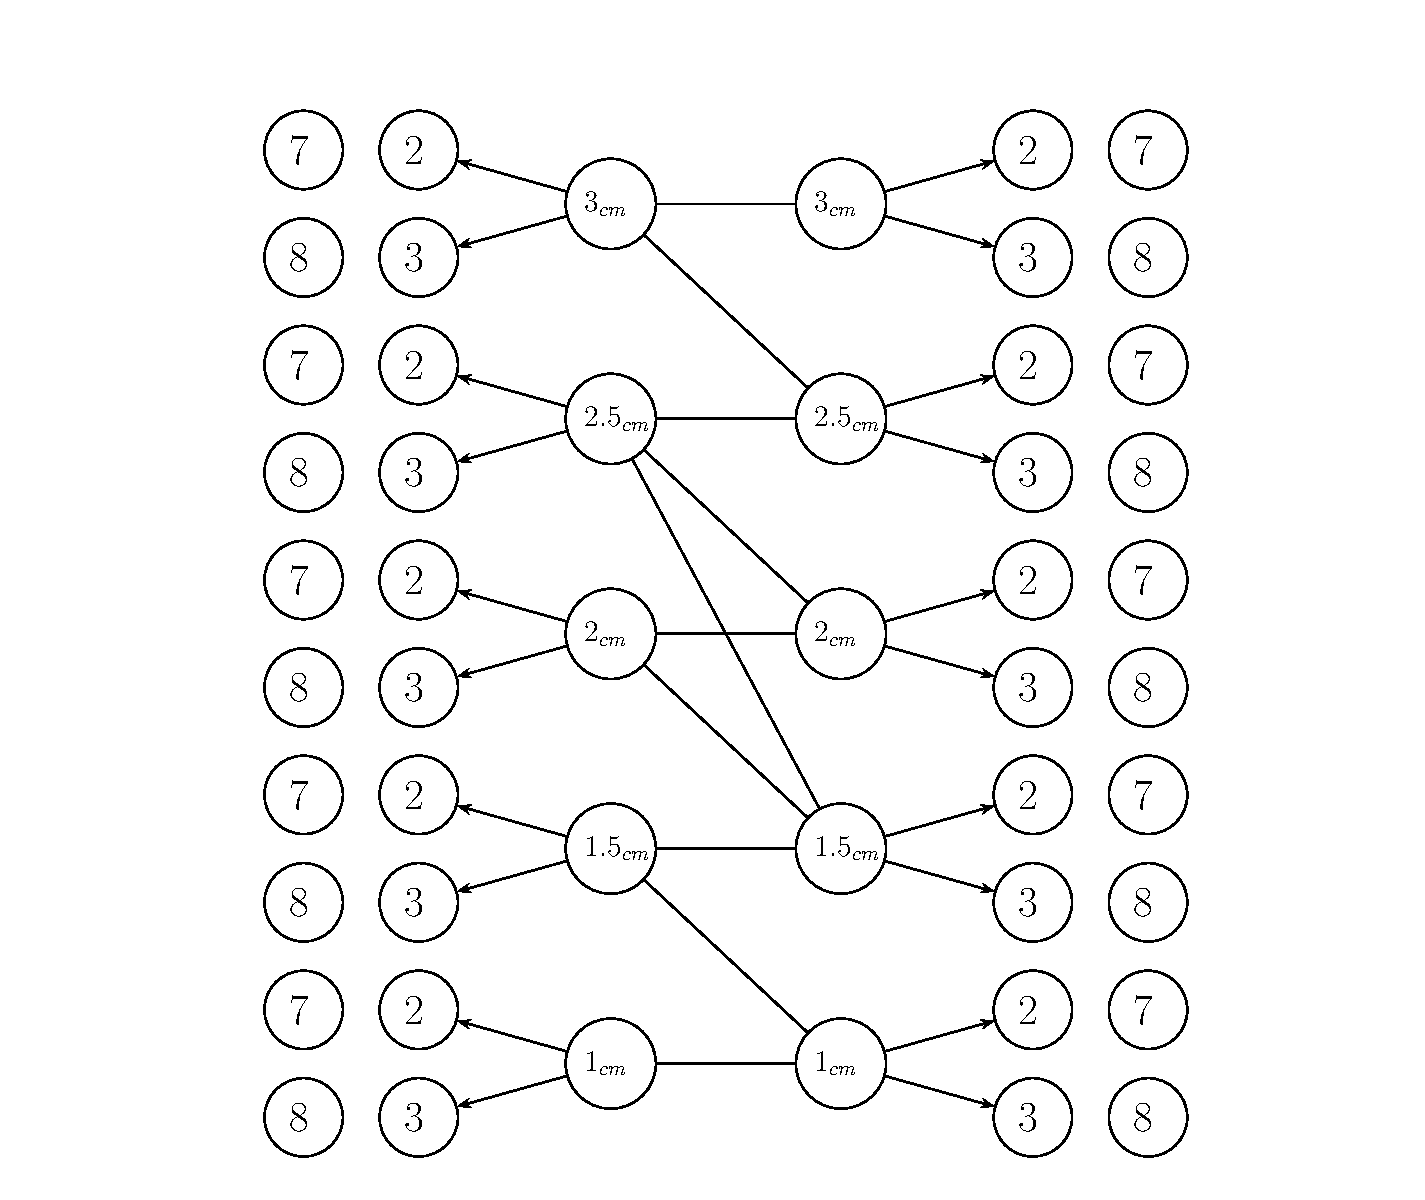
\includegraphics[width=0.99\textwidth]{Figures/Estimulos_Experimento2} 
\decoRule
\caption[Diseño de Estimulos en el Experimento 2]{Diseño de las parejas  de figuras de Ebbinghaus a comparar en el Experimento 2. Se manejaron cinco tamaños distintos de círculo central, que se mostraron en parejas iguales (cinco señales) y cinco parejas desiguales (cuatro cuyos círculos centrales diferían en 0.5 cm y, una con una diferencia de 1 cm). En cada pareja siempre había una figura de Ebbinghaus que inducía la subestimación del tamaño central y una que promovía la subestimación, contrabalanceando el orden en que aparecían en pantalla (relativo a la posición izquierda o derecha). Por cada pareja de círculos centrales, se contemplaron cuatro combinaciones posibles entre los dos niveles de círculos externos contenidos por cada condición (i.e. a vs a, b vs b, a vs b, b vs a; donde a y b son sustituíbles por 2 y 3 círculos externos en la condición fácil o 7 y 8, en la condición difícil.)}
\label{fig:Exp_2}
\end{figure}

\end{itemize}





\subsection{Materiales}

%Programacion de la tarea
La tarea fue programada y ejecutada en PsychoPy v.12, un paquete de libre acceso programado en lenguaje Python que facilita la generación de experimentos en psicología y neurociencia.

%Lugar de ejecución
El experimento se corrió en una computadora Mac, con una pantalla de $medidas$, en un cubículo donde se procuró que los participantes permanecieran aislados, dentro del laboratorio 25 del Edificio D de la Facultad de Psicología de la UNAM.

\subsection{Participantes}

%Total de participantes y distribucion entre experimentos.
Un total de cuarenta y un estudiantes de la Facultad de Psicología participaron en alguno de los dos experimentos planteados: veinte en el Experimento 1 y veintiuno en el Experimento 2. Los experimentos se llevaron a cabo de manera simultáneá. Los participantes fueron asignados a ambos experimentos de manera alternada, con el propósito de terminar con una muestra de participantes similar entre estos.\\

%Consentimiento informado y acuerdos
Todos los participantes fueron estudiantes de los primeros cuatro semestres de la licenciatura en Psicología en la Facultad de Psicología de la Universidad Nacional Autónoma de México; sus edades variaban entre los 18 y los 21 años. Los participantes fueron invitados a participar a cambio de entrar en una rifa donde podrían ganar una tarjeta de regalo con valor de $\300.00$ pesos para la plataforma de su preferencia entre iTunes, Netflix y Amazon. Se realizó una rifa independiente por cada experimento.\\ 

Antes de participar en el experimento, se solicitó a cada participante que firmara una carta de consentimiento individual donde se les informaba la duración estimada de la tarea (40 minutos para cualquiera de los experimentos), se les advertía que el procedimiento podría resultar fatigoso y que, aunque su participación era voluntaria y podían dimitir en cualquier momento, su permanencia en el mismo hasta el final era crucial para poder utilizar sus datos, y se reafirmaba su participación en una de las rifas. Los participantes proporcionaron teléfonos y correos como medio de contacto.\\

\section{Procedimiento}

%Descripcion del procedimiento



%Controles
Se controló que la distancia que separase los estímulos presentados se encontrara dentro de un ángulo de $X grados$ del campo visual de los participantes, así como que estos realizaran la tarea en una distancia de 1 m respecto del monitor.



\subsection{Registro de respuestas}

El experimento fue programado de manera tal que por cada participante se obtuviera un documento en formato csv (i.e. comma separated value) que contuviera información, ensayo a ensayo, sobre la respuesta dada por 
